\section{Auswertung}
\label{sec:Auswertung}

\subsection{Fourier-Analyse}

Die gemessenen Amplituden der drei Spannungen $U_R$ (Rechteck), $U_S$ (Sägezahn) und $U_D$ (Dreieck), werden in den Tabellen 1,2 und 3 dargestellt.
Die Quotienten $\frac{U_n}{U_1}$ werden ebenfalls in den tabellen dargestellt, da diese für
spätere Rechnungen nötig sind.
 Die Frequenz des Funktionsgenerators beträgt bei allen Messungen $1$kHz.

\begin{table}[H]
  \centering
  \caption{Amplituden und Frequenzen der Rechteckspannung}
  \label{tab:Rechteckspannung}
  \begin{tabular}{c c | c c | c c}
    \toprule
    $U_R/V$ & $\frac{U_n}{U_1}$ & $U_S/V$ & $\frac{U_n}{U_1}$ & $U_D/V$ & $\frac{U_n}{U_1}$ \\
    \midrule
    4.44 & 1.00 & 2.18 & 1.00 & 2.80 &  1.00 \\
    1.36 & 0.31 & 1.04 & 0.48 & 0.30 &  0.11\\
    0.72 & 0.16 & 0.64 & 0.29 & 0.10 &  0.04\\
    0.56 & 0.13 & 0.44 & 0.20 & 0.05 &  0.02\\
    0.48 & 0.11 & 0.30 & 0.14 & 0.03 &  0.01\\
    0.40 & 0.09 & 0.26 & 0.12 & 0.02 &  0.01\\
    0.32 & 0.07 & 0.24 & 0.11 & 0.02 &  0.01\\
    0.24 & 0.05 & 0.20 & 0.09 & 0.01 &  0.00\\
    0.24 & 0.05 & 0.18 & 0.08 & 0.01 &  0.00\\
    \bottomrule
  \end{tabular}
\end{table}

Der Logarithmus von $\left( \frac{U_n}{U_1}\right)$ der drei Spannungen wird gegen $n$ aufgetragen.

\begin{figure}
  \centering
  \includegraphics{plot1.pdf}
  \caption{Lineare Regression der Rechteckschwingung}
  \label{fig:rechteck}
\end{figure}

Die Gerade wird durch die Gleichung $y = m_1x + b_1$ beschrieben. Die Parameter betragen:
\begin{align*}
  m_1 &= -1.32 \pm 0.07 \\
  b_1 &= -0.16 \pm 0.10
\end{align*}

Der Theoriewert beträgt $m_1=-1$. Die relative Abweichung des berechneten Wertes von dem Theoriewert beträgt 32.0\%.

\begin{figure}
  \centering
  \includegraphics{plot2.pdf}
  \caption{Lineare Regression der Sägezahnschwingung}
  \label{fig:saegezahn}
\end{figure}

Die Gerade wird durch die Gleichung $y = m_2x + b_2$ beschrieben. Die Parameter betragen:
\begin{align*}
  m_1 &= -1.17 \pm 0.03 \\
  b_1 &= 0.02 \pm 0.04
\end{align*}

Der Theoriewert beträgt $m_2=-1$. Die relative Abweichung des berechneten Wertes von dem Theoriewert beträgt 17.0\%.

\begin{figure}[H]
  \centering
  \includegraphics{plot3.pdf}
  \caption{Lineare Regression der Dreieckschwingung}
  \label{fig:dreieck}
\end{figure}

Die letzten beiden Messwerte werden, wegen zu kleiner Amplitude, nicht in dem Plot berücksichtig.
Die Gerade wird durch die Gleichung $y = m_2x + b_2$ beschrieben. Die Parameter betragen:
\begin{align*}
  m_1 &= -2.45 \pm 0.21 \\
  b_1 &= 0.32 \pm 0.29
\end{align*}

Der Theoriewert beträgt $m_3=-2$. Die relative Abweichung des berechneten Wertes von dem Theoriewert beträgt 22.5\%.

\subsection{Fourier-Synthese}
Abbildung 5,6 und 7 stellen die synthetisierten Schwingungen dar.

\begin{figure}[H]
  \centering
  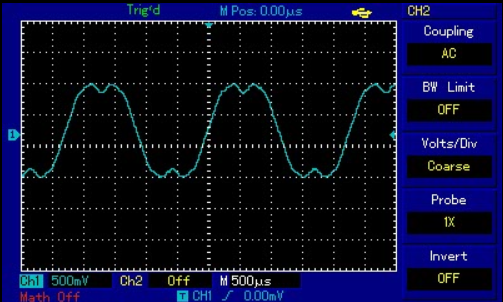
\includegraphics[height=5cm]{rechteck.PNG}
  \caption{Synthetisierte Rechteckschwingung}
  \label{fig:rechteck}
\end{figure}


\begin{figure}[H]
  \centering
  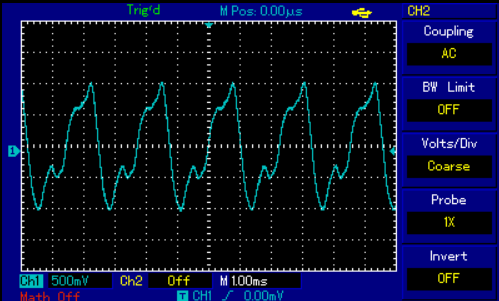
\includegraphics[height=5cm]{saegezahn.PNG}
  \caption{Synthetisierte Sägezahnschwingung}
  \label{fig:saegezahn}
\end{figure}


\begin{figure}[H]
  \centering
  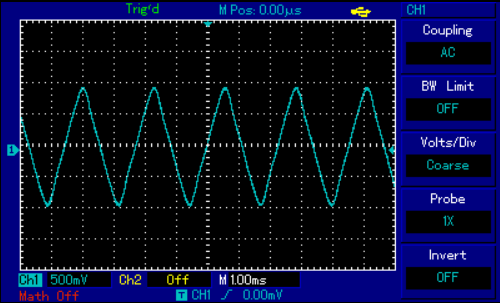
\includegraphics[height=5cm]{dreieck.PNG}
  \caption{Synthetisierte Dreieckschwingung}
  \label{fig:dreieck}
\end{figure}
